\acrlongpl{gnn} have become fundamental to \acrlong{dl} field, particularly for tasks involving non-Euclidean data structures.
These models have had a significant impact on several domains, such as social network analysis, bioinformatics, recommender systems and \gls{nlp}.
This section explores the development, key architectures, methodologies, applications and methodologies, applications, challenges and future directions of \glspl{gnn}.

\subsection*{Historical Context and Evolution}

\subsubsection*{Early Work and Foundations}

Graphs have received success because the achievements of neural networks, for \gls{ml} tasks such as object detection and speech recognition.
Graphs are mathematical structures consisting of nodes connected by edges, making them ideal for modeling relationships and dependencies in complex systems.
Mathematically, a graph is defined as $G=(V, E)$, where $V$ represents the nodes and $E$ represents the edges. The edges in a graph can be either directed or undirected, depending on whether directional dependencies exist between the nodes.
Graphs are used to represent real-world datasets like protein-protein interaction networks, social networks, traffic forecasting, e-commerce, geographical maps, \glspl{kg} and so on.
\\\glspl{gnn} draw inspiration from \glspl{cnn}.
According to \cite{Khemani2024}, \glspl{cnn} and \glspl{rnn} are not well-suited for effectively handling graph-structured data.
\glspl{cnn} are designed for data with a grid structure, such as images, while \glspl{rnn} are tailored for sequences, like text.
Typically, arrays are used for storing text data, and matrices are used for image data. However, arrays and matrices are inadequate for dealing with graph data.
For graphs, we need a specialized technique called Graph Convolution. This technique allows deep neural networks to process graph-structured data directly, resulting in a \glspl{gnn}.
Nowadays, however there is a continuous increase in applications and domains that use complex structures such as graphs (\cite{Wu2021}).
The complexity of graphs implied not insignificant problems on existing \gls{ml} algorithms because a graph may have a variable number of nodes or edges; or it might have nodes that may have a different number of neighbours.
This last point is very important in some operation like convolution, that is easy for images but not for graphs.
Another motivation comes from graph representation learning, which aims to learn to represent graph nodes, edges or subgraphs by low-dimensional vectors (\cite{Zhou2020}).
Existing word embedding methods like DeepWalk (\cite{Perozzi2014}), node2vec (\cite{Grover2016}), LINE (\cite{Tang2015}) have achieved very good results but they have 2 important drawbacks. The first one is that there are no shared parameters in the encoder, which implies computationally inefficency (n. of parameters grows linearly with the n. of nodes);
The second drawback is that there's a lack of generalization because they cannot deal with dynamic graphs or generalize to new graphs.
\\Inspired by the success of \glspl{cnn} and \glspl{rnn}, \cite{Gori2005, Scarselli2009} have designed and developed the first \gls{gnn} model in order to operate on non-Euclidian space.
Variations of \glspl{gnn}, including \glspl{gcn}, \glspl{gat}, and GraphSAGE, have demonstrated groundbreaking performance on various \gls{dl} tasks in recent years.
\\To summarize, a \gls{gnn} aims to learn a state embedding \( h_v \in \mathbb{R}^s \) that encapsulates the neighborhood data of each node.
This state embedding \( h_v \), an $s$-dimensional vector for node \( v \), can be used to generate an output \( O_v \), such as the predicted distribution of the node label.
The predicted node label distribution (\( O_v \)) is derived from the state embedding \( h_v \) (\cite{Rong2019}).

\subsection*{GNN Learning Tasks and Training Settings}
According to \cite{Zhou2020,Wu2021}, \glspl{gnn} are versatile tools capable of performing a variety of node-level, edge-level, and graph-level tasks.
Each approach leverages different amounts and types of labeled data to extract meaningful patterns and representations from graph-structured data.
These approaches are described below.
Fig. \ref{fig:gnn-graph-learning-tasks-summary} summarizes the key graph learning tasks that \glspl{gnn} can perform, highlighting the diversity and flexibility of these models in handling various types of graph-structured data.

\textbf{Node-level} tasks focus on predicting or inferring properties of individual nodes within a graph. This includes node classification, where each node is classified into one of several predefined categories, and node regression, which predicts continuous values associated with nodes.
Node clustering groups nodes into clusters based on feature similarity and structural proximity, and node representation learning focuses on learning low-dimensional embeddings that preserve the graph's structural and feature information.

\textbf{Edge-level} tasks aim to predict or infer properties related to the edges in a graph.
Link prediction involves predicting the existence of an edge between two nodes and is crucial for applications such as recommending friends in social networks or predicting interactions in biological networks.
Edge classification assigns categories to edges based on the properties of the connected nodes and their relationships, while edge regression predicts continuous values associated with edges, such as the strength of interactions or the weight of connections.

\textbf{Graph-level} tasks involve making predictions or inferences about entire graphs.
Graph classification assigns a label to an entire graph, which is useful in applications like classifying molecules or categorizing social networks.
Graph regression predicts continuous values for entire graphs, such as the bioactivity of chemical compounds or the performance metrics of network designs.
Graph generation involves creating new graphs that resemble a given set of graphs and is important in applications like molecule generation for drug discovery or network topology design.

\begin{figure}[htbp]
    \centering
 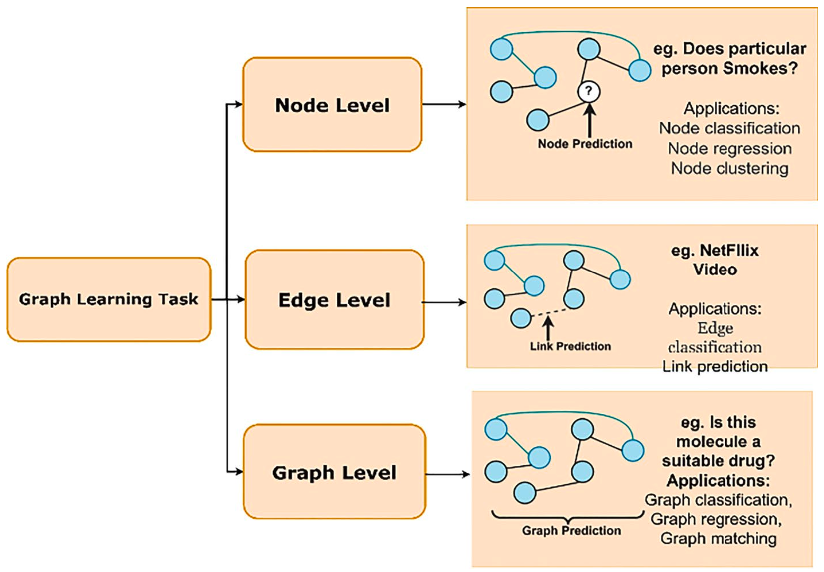
\includegraphics[width=.9\textwidth]{03_Figures/literature-review/gnn-graph-learning-tasks-summary.png}
     \rule{35em}{0.5pt}
    \caption{Graph learning tasks by \glspl{gnn} (\cite{Khemani2024})} 
 \label{fig:gnn-graph-learning-tasks-summary}
\end{figure}

\glspl{gnn} can be trained using a variety of learning paradigms, including supervised, semi-supervised, or unsupervised learning approaches, each of which leverages different methods and data availability to optimize the model for various analytical tasks on graph-structured data (\cite{Zhou2020,Wu2021}).

In \textbf{supervised learning}, models are trained using labeled data, where each input example is paired with the correct output.
For \glspl{gnn}, supervised tasks include node classification, link prediction, and graph classification, with a loss function defined based on the difference between predicted and actual labels.

\textbf{Semi-supervised learning} uses a small amount of labeled data along with a large amount of unlabeled data (\cite{Kipf2017}).
\glspl{gnn} are well-suited for this approach due to their ability to leverage graph structure and propagate label information through the network.
Semi-supervised tasks include semi-supervised node classification and semi-supervised link prediction, allowing models to make use of the vast amounts of unlabeled data, which is often easier and cheaper to obtain.

\textbf{Unsupervised learning} involves training a model without any labeled data, relying solely on the structure and inherent properties of the input data.
In \glspl{gnn}, unsupervised tasks include node clustering, graph embedding, and graph generation.
Techniques like autoencoders, where the model learns to reconstruct the input graph from compressed embeddings, or contrastive learning, where the model learns representations by contrasting positive and negative samples derived from the graph structure, are often used in unsupervised learning.

\subsection*{The Message-Passing Mechanism}
The message-passing mechanism in \glspl{gnn} is a sophisticated process that maintains graph symmetries through optimizable transformations on all graph properties, including nodes, edges, and the global context, preserving permutation invariances (\cite{Khemani2024}).
This ensures that the connectivity of the input graph remains unchanged, allowing the output to be characterized using the same adjacency list and feature vector count as the input.
However, the output graph has updated embeddings as the \gls{gnn} modifies each node, edge, and global-context representation.

At its core, the message-passing mechanism operates iteratively, enabling nodes to collect and aggregate information from their neighbors.
According to \cite{Khemani2024}, the message-passing mechanism in \glspl{gnn} involves the following key steps:
\begin{enumerate}
    \item \textbf{Node Representation Initialization}: each node in the graph is initialized with a feature vector. These initial representations can be based on node attributes or initialized randomly.

    \item \textbf{Message Passing Phase}: this phase involves multiple iterations, during which nodes exchange and aggregate information from their neighbors. The process unfolds as follows:
    \begin{itemize}
        \item[a.] \textbf{Message Computation}: each node generates a message to be sent to its neighboring nodes. This message is typically a function of the node's current feature vector and the feature vectors of its neighbors. Formally, for a node \(u\), the message \(m_{u}^{(k)}\) sent to its neighbors can be computed using a differentiable function such as a neural network:
        \[
        m_{u}^{(k)} = MessageFunction(h_u^{(k)}, \{h_v^{(k)}~|~v \in \mathcal{N}(u)\}, \{e_{uv}~|~v \in \mathcal{N}(u)\})
        \]
        where \(h_u^{(k)}\) is the feature vector of node \(u\) at iteration \(k\), \(\mathcal{N}(u)\) denotes the neighbors of node \(u\), and \(e_{uv}\) represents the edge features between nodes \(u\) and \(v\).
  
        \item[b.] \textbf{Message Aggregation}: each node aggregates the messages received from its neighbors. The aggregation function is typically permutation-invariant, ensuring that the order of the neighboring nodes does not affect the result. Common aggregation functions include summation, mean, or max. For a node \(u\), the aggregated message \(M_u^{(k)}\) is computed as:
        \[
        M_u^{(k)} = AGGREGATE^{(k)}(\{m_{v}^{(k)}~|~v \in \mathcal{N}(u)\})
        \]
  
        \item[c.] \textbf{Node Update}: each node updates its feature vector based on the aggregated message and its current feature vector. This update is performed using an update function, often a neural network. For a node \(u\), the updated feature vector \(h_u^{(k+1)}\) is computed as:
        \[
        h_u^{(k+1)} = UPDATE^{(k)}(h_u^{(k)}, M_u^{(k)})
        \]
    \end{itemize}

    \item \textbf{Iteration and Neighborhood Expansion}: the message-passing phase is repeated for multiple iterations. With each iteration, nodes accumulate information from increasingly distant parts of the graph. After the first iteration (\(k=1\)), each node's embedding includes information from its 1-hop neighborhood. After the second iteration (\(k=2\)), each node's embedding incorporates information from its 2-hop neighborhood, and so on. Generally, after \(k\) iterations, each node's embedding contains data from its \(k\)-hop neighborhood.

    \item \textbf{Structural and Feature-Based Information}: the information passed during message passing consists of two main components: structural information about the graph (such as the degree of nodes) and feature-based information (attributes of the nodes and edges). Each node's message is stored in the form of feature vectors, and during each iteration, these vectors are updated to reflect the aggregated information from neighboring nodes.

    \item \textbf{Readout Phase}: after completing the message-passing iterations, a readout function is applied to extract the final representation for nodes, edges, or the entire graph. This function aggregates the final node embeddings into a single representation. For graph-level tasks, the readout function might be a global pooling operation, such as summation, mean, or max over all node feature vectors.
\end{enumerate}

The entire process can be mathematically represented as:
   \[
   h_u^{(k+1)} = UPDATE^{(k)}\left(h_u^{(k)}, AGGREGATE^{(k)}\left(\{m_{v}^{(k)}~|~v \in \mathcal{N}(u)\}\right)\right)
   \]
where \(h_u^{(k)}\) denotes the feature vector of node \(u\) at iteration \(k\), and \(m_{v}^{(k)}\) represents the message from node \(v\) at iteration \(k\). The AGGREGATE function combines the messages from the neighbors, and the UPDATE function combines this aggregated message with the node's current feature vector to produce the updated feature vector.

The message-passing mechanism of \glspl{gnn} is illustrated Fig. \ref{fig:gnn-message-passing-mechanism}.
Here, an input graph with a set of node features \(X \in \mathbb{R}^{d \times |V|}\) is used to produce updated node embeddings.
The process begins with each node having an initial message (or feature vector).
Nodes then exchange messages with their neighbors. For instance, the B user node collects messages from its neighboring nodes, which are then aggregated.
This aggregated message is used to update B user's node feature vector, resulting in a new embedding for the B user node for the next iteration.
The diagram visually represents how messages are computed, aggregated, and updated across nodes in the graph, leading to refined node embeddings over iterations.

\begin{figure}[htbp]
    \centering
 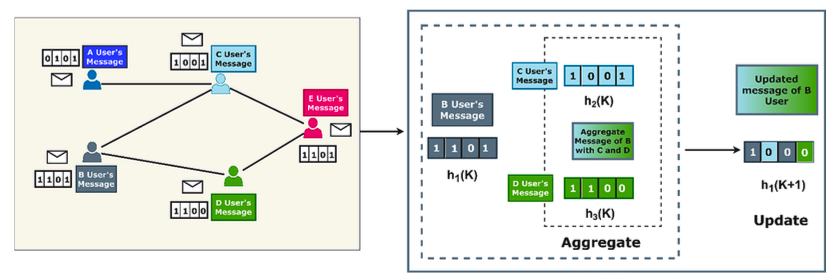
\includegraphics[width=.9\textwidth]{03_Figures/literature-review/gnn-message-passing-mechanism.png}
     \rule{35em}{0.5pt}
    \caption{Message passing mechanism in \glspl{gnn} (\cite{Khemani2024})} 
 \label{fig:gnn-message-passing-mechanism}
\end{figure}

This mechanism enables \glspl{gnn} to effectively capture the dependencies and relationships within graph-structured data, making them powerful tools for tasks like node classification, link prediction, and graph classification.
By iteratively exchanging and aggregating information, \glspl{gnn} can learn rich, expressive representations that reflect both the structure and attributes of the graph.

\subsection*{\gls{gnn} Models}
Over the years, different models of \glspl{gnn} have been developed, each with its own potential and for specific tasks.
The following are the most important and best-known network architectures in the literature.

\subsubsection*{Spectral Approaches}

The breakthrough in spectral approaches marked a significant evolution in \glspl{gnn}. \cite{Bruna2013} introduced a method leveraging spectral graph theory to define convolution operations on graphs. This approach was refined by \cite{Defferrard2016}, leading to more efficient models. \cite{Kipf2017} simplified this concept further, making it more accessible and practical, thus popularizing the \gls{gcn}.

\subsubsection*{\acrfullpl{gcn}}

%\glspl{gcn} represent one of the most influential architectures in the \gls{gnn} landscape. They generalize the convolution operation to graph data, enabling the aggregation of feature information from a node's neighbors.
\glspl{gcn} are a fundamental variant of graph neural networks developed by \cite{Kipf2017}.
The convolution layers in \glspl{gcn} operate similarly to the convolution process in \glspl{cnn}.
In \glspl{cnn}, input neurons are multiplied by weights known as filters or kernels, which act as a sliding window across the image, allowing the network to learn from nearby cells.
Weight sharing involves using the same filter throughout the same layer of the image.
For instance, when \glspl{cnn} are used to distinguish between images of cats and non-cats, the same filter detects the cat's nose and ears across the image.
This concept applies to \glspl{gcn} as well, where similar filters are applied throughout the graph structure (\cite{Kipf2017}).

\glspl{gcn} operate by learning features through the analysis of neighboring nodes, mirroring the behavior of \glspl{cnn}.
However, the primary distinction between \glspl{cnn} and \glspl{gnn} lies in their application domains: \glspl{cnn} are designed to handle regular, Euclidean-ordered data, while \glspl{gnn} are a generalized form of CNNs suited for irregular, non-Euclidean data with varying numbers of node connections and unordered nodes.
They extend traditional \glspl{cnn}, which are typically used for grid-like data such as images, by performing convolution operations on graph data.
This enables \glspl{gcn} to capture and propagate information through the graph's nodes, considering both a node's features and those of its neighbors.
\glspl{gcn} have been successfully applied to various problems, including image classification (\cite{Monti2016}), traffic forecasting (\cite{Cui2020}), recommendation systems (\cite{Fan2019}) and scene graph generation (\cite{Yang_2018_ECCV}).

\glspl{gcn} consist of multiple layers, each performing convolution and aggregation steps to refine node representations.
By iteratively applying these layers, \glspl{gcn} can capture complex patterns and dependencies within the graph data.
Fig. \ref{fig:gcn-semisupervised-learning} illustrates a multi-layer \gls{gcn} for semi-supervised learning task.

A \gls{gcn} layer can be formally represented as:

\[ H^{(l+1)} = \sigma\left(\tilde{D}^{-\frac{1}{2}}\tilde{A}\tilde{D}^{-\frac{1}{2}} H^{(l)} W^{(l)}\right) \]

where:
\begin{itemize}
    \item \( \tilde{A} = A + I \) is the adjacency matrix with added self-loops.
    \item \( \tilde{D} \) is the degree matrix of \( \tilde{A} \).
    \item \( H^{(l)} \) and \( H^{(l+1)} \) are the input and output feature matrices for layer \( l \).
    \item \( W^{(l)} \) is the trainable weight matrix.
    \item \( \sigma \) is an activation function like ReLU.
\end{itemize}

\begin{figure}[htbp]
    \centering
 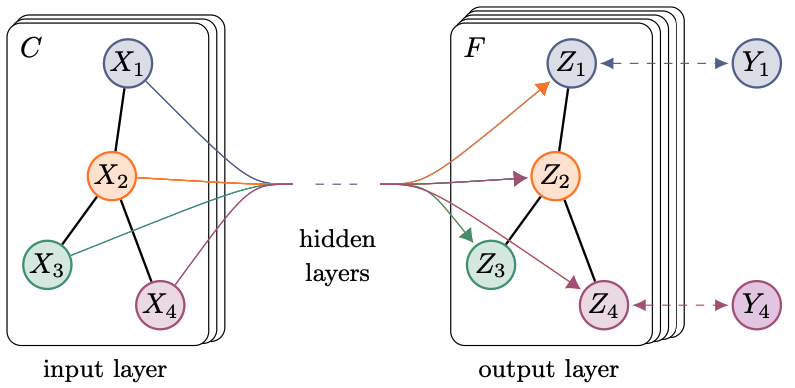
\includegraphics[width=.7\textwidth]{03_Figures/literature-review/gcn-semisupervised-learning.png}
     \rule{35em}{0.5pt}
    \caption{Schematic representation of a multi-layer \gls{gcn} for semi-supervised learning with $C$ input channels and $F$ feature maps in the output layer.  (\cite{Kipf2017})} 
 \label{fig:gcn-semisupervised-learning}
\end{figure}

\glspl{gcn} offer several advantages.
One key advantage is their ability to naturally handle graph-structured data, making them well-suited for tasks involving complex relational structures.
\glspl{gcn} leverage the connectivity information in graphs to capture and propagate node features, enabling more effective learning from the data's inherent structure.
This capability extends the powerful concept of convolution from Euclidean data, like images, to non-Euclidean data, such as graphs, allowing for a more generalized application of neural network models (\cite{Wu2021}).
Additionally, \glspl{gcn} are computationally efficient for large-scale graph data, as they utilize localized operations that limit the complexity of processing entire graphs at once.
This localized approach helps in scaling \glspl{gcn} to larger datasets and complex networks (\cite{Li2018}).

However, \glspl{gcn} also have limitations.
One major limitation is their reliance on the assumption of homophily, where connected nodes are assumed to have similar features.
This can restrict their effectiveness in graphs where such an assumption does not hold, such as in heterophilic graphs where connected nodes may have dissimilar features (\cite{Xu2019}).
Another limitation is the potential for oversmoothing, where node features become indistinguishable after several layers of convolution, leading to a loss of meaningful differentiation between nodes.
This can hinder the model's ability to capture fine-grained information in deeper architectures (\cite{Li2018}).
Additionally, \glspl{gcn} often struggle with scalability in extremely large graphs or dynamic graphs where the structure changes frequently, as the need to recompute convolutions can become computationally intensive.
Finally, \glspl{gcn} require careful tuning of hyperparameters and can be sensitive to the choice of architecture, which may limit their accessibility and ease of use for practitioners without extensive expertise in \glspl{gnn} (\cite{Wu2021}).

\subsubsection*{\acrfullpl{gat}}

\cite{Velickovic2018} introduced \glspl{gat}, which incorporate attention mechanisms to dynamically weigh the importance of neighboring nodes.
\gls{gat} is a novel neural network designed to work with graph-structured data.
It employs masked self-attentional layers to overcome the limitations of previous methods that relied on graph convolutions or their approximations.
By stacking these layers, \gls{gat} enables the model to implicitly assign different weights to various nodes in a neighborhood, allowing nodes to focus on the most relevant features of their neighbors.
This approach eliminates the need for expensive matrix operations, such as inversion, and does not require prior knowledge of the graph's structure.
\gls{gat} effectively addresses many significant limitations of spectral-based graph neural networks, making the model suitable for both inductive and transductive tasks.

The attention mechanism is formally defined as follows:

\[ e_{ij} = \text{LeakyReLU}\left(a^T [W h_i \| W h_j]\right) \]

where \( e_{ij} \) is the attention score, \( a \) is the learnable attention vector, and \( \| \) denotes concatenation.

\[ \alpha_{ij} = \frac{\exp(e_{ij})}{\sum_{k \in \mathcal{N}(i)} \exp(e_{ik})} \]

The node features are updated as:

\[ h_i' = \sigma\left(\sum_{j \in \mathcal{N}(i)} \alpha_{ij} W h_j\right) \]

Fig. \ref{fig:gat-attention-mechanism} shows the coefficients computed by the attention mechanism, parametrized by a weight vector $\vec{\mathbf{a}} \in \mathbb{R}^{2F}$ (where $F$ is the number of features in each node), applying a LeakyReLU activation.
\begin{figure}[htbp]
    \centering
 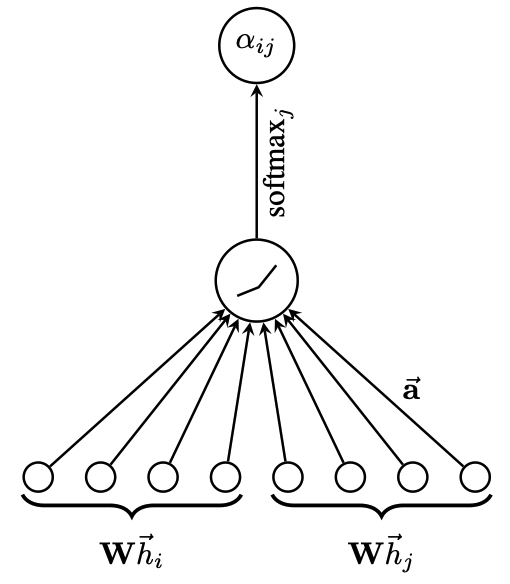
\includegraphics[width=.3\textwidth]{03_Figures/literature-review/gat-attention-mechanism.png}
     \rule{35em}{0.5pt}
    \caption{Attention mechanism in \glspl{gat} (\cite{Velickovic2018})} 
 \label{fig:gat-attention-mechanism}
\end{figure}


\glspl{gat} provide numerous advantages.
One of the main benefits is their capability to assign different importance weights to nodes within a neighborhood, enhancing the model's ability to concentrate on the most relevant features and relationships.
This is facilitated by the self-attention mechanism, which avoids the need for expensive matrix operations or prior knowledge of the graph's structure, thus making \glspl{gat} computationally efficient and versatile (\cite{Velickovic2018}).
Furthermore, \glspl{gat} can naturally manage graphs with varying node degrees and adapt to different scales, offering robustness and scalability.
The ability to learn dynamic attention weights for different nodes makes \glspl{gat} especially effective for tasks involving heterogeneous graphs and those with complex, irregular structures.

Nevertheless \glspl{gat} also have certain limitations.
A notable challenge is that the attention mechanism can be computationally demanding, especially for large-scale graphs with numerous nodes and edges, potentially causing scalability issues.
The computational complexity of the self-attention mechanism can grow with the number of nodes, making it less efficient for very large graphs compared to simpler convolutional methods (\cite{Thekumparampil2018}).
Additionally, although \glspl{gat} can focus on relevant nodes, they may suffer from overfitting, particularly when the attention mechanism excessively emphasizes specific nodes, leading to a reduction in generalization.
Furthermore, tuning the hyperparameters of the attention mechanism can be intricate and requires careful experimentation to achieve optimal performance (\cite{Lee2018}).

\subsubsection*{GraphSAGE}

\gls{graphsage} is an inductive learning framework for graph-structured data.
Unlike traditional methods that rely on transductive learning, \gls{graphsage} focuses on generalizing to unseen nodes, making it well-suited for dynamic graphs or scenarios where the graph structure evolves over time (\cite{Hamilton2017}).
This network consists of two main steps: Sampling and Aggregation, followed by a node representation update and normalization step.
Below, these steps are briefly described
Sampling, aggregating and predicting steps are illustrated in Fig. \ref{fig:graphsage-approach}.


\begin{enumerate}
    \item \textbf{Sampling}: in the sampling step, \gls{graphsage} samples a fixed-size set of neighbors for each node. This helps manage the complexity of the graph by limiting the number of neighbors considered during aggregation. Formally, for a node \(v\), a fixed-size set of neighbors \(\mathcal{N}(v)\) is sampled:
    \[
    \mathcal{N}(v) \subseteq \{u \in V~|~(v, u) \in E\}
    \]
 
    \item \textbf{Aggregation}: the aggregation step involves aggregating the feature vectors of the sampled neighbors to generate an updated representation for the node. Several aggregation functions can be used, including mean, LSTM-based, and pooling aggregators. The aggregation function is denoted as:
    \[
    h_{\mathcal{N}(v)}^{(k)} = \text{AGGREGATE}^{(k)}(\{h_u^{(k-1)}, \forall~u \in \mathcal{N}(v)\})
    \]
    where \(h_u^{(k-1)}\) is the representation of node \(u\) at the \((k-1)\)-th layer.
 
    \item \textbf{Update}: after aggregation, the node's representation is updated by combining its current representation with the aggregated neighborhood information. This is followed by a nonlinear transformation using a weight matrix and an activation function, such as ReLU:
    \[
    h_v^{(k)} = \sigma\left(W^{(k)} \cdot \text{CONCAT}(h_v^{(k-1)}, h_{\mathcal{N}(v)}^{(k)})\right)
    \]
    where \(W^{(k)}\) is the weight matrix for the \(k\)-th layer and \(\sigma\) is a nonlinear activation function.
 
    \item \textbf{Normalization}: finally, a normalization step is applied to ensure stability and prevent exploding or vanishing gradients. This is typically done using L2 normalization:
    \[
    h_v^{(k)} = \frac{h_v^{(k)}}{\|h_v^{(k)}\|}
    \]
\end{enumerate}

\begin{figure}[htbp]
    \centering
 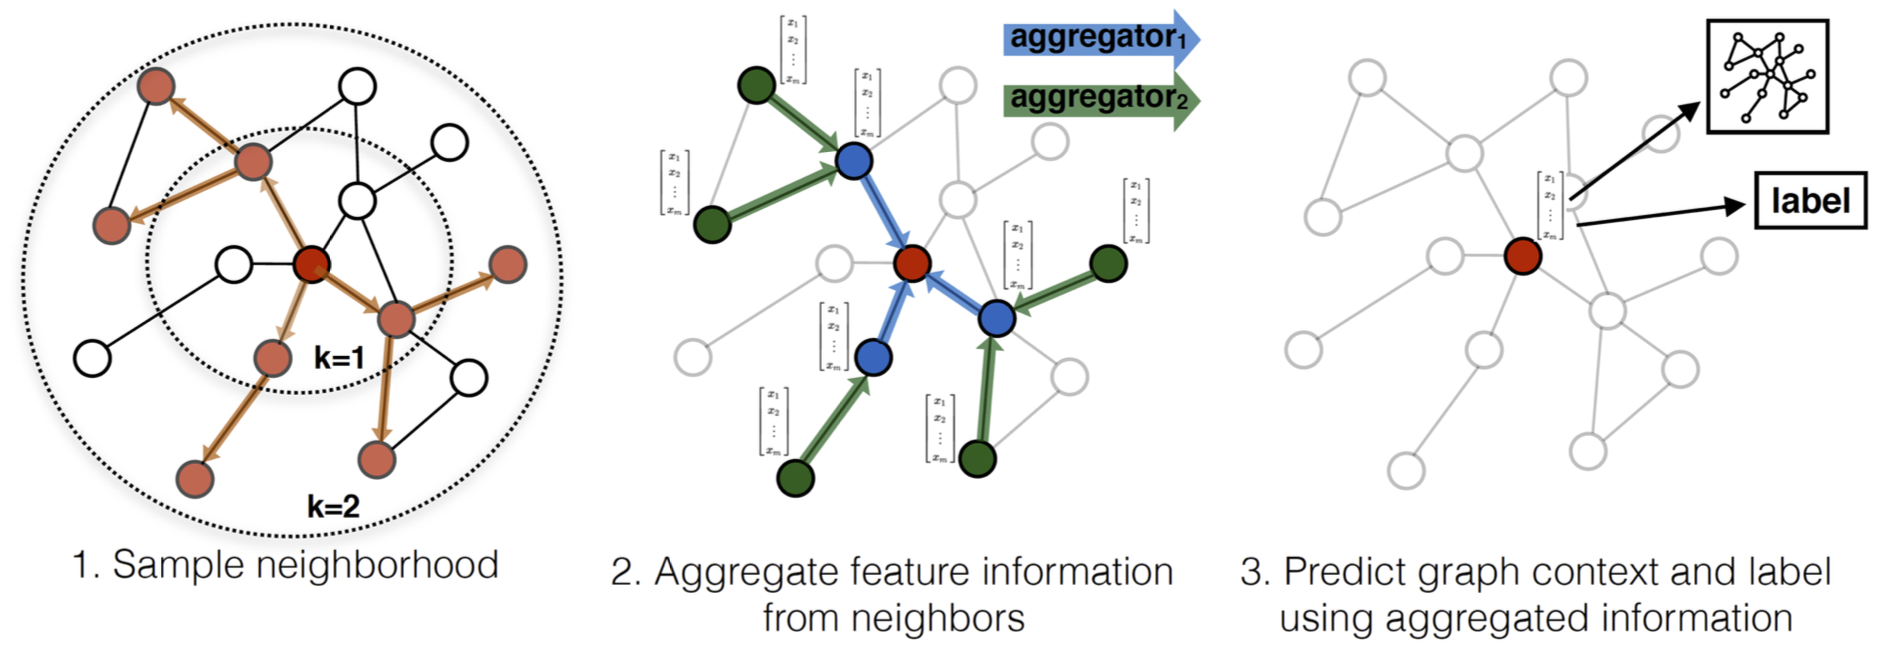
\includegraphics[width=.9\textwidth]{03_Figures/literature-review/graphsage-approach.png}
     \rule{35em}{0.5pt}
    \caption{Visual working of the \gls{graphsage} sampling and aggregation approach. (\cite{Hamilton2017})} 
 \label{fig:graphsage-approach}
\end{figure}

\gls{graphsage} has several advantages.
One key advantage is its ability to generalize to unseen nodes, making it suitable for inductive tasks.
This is particularly useful in dynamic graphs where new nodes and edges continuously emerge (\cite{Hamilton2017}).
Additionally, the sampling step significantly reduces computational complexity, enabling the model to scale to large graphs.
The flexibility of the aggregation function allows for customization based on specific applications, and the use of multiple layers facilitates the capture of higher-order neighborhood information.

Despite its advantages, \gls{graphsage} also has limitations.
The sampling process may lead to information loss, as only a subset of neighbors is considered.
This can affect the quality of the learned representations, especially in sparse graphs.
Additionally, the choice of the aggregation function and hyperparameters can significantly impact performance, requiring careful tuning.
Another limitation is that while \gls{graphsage} is designed to handle large-scale graphs, it may still face challenges with extremely large or highly dynamic graphs where the graph structure changes rapidly (\cite{Wu2021}).

\subsubsection*{Other \gls{gnn} models}

\glspl{mpnn} are a class of neural networks specifically designed for graph-structured data.
\glspl{mpnn} use a framework where nodes iteratively exchange and aggregate information.
Each node's state is updated by aggregating messages from its neighbors and applying an update function to these messages along with the node's current state.
The message function generates messages from the feature vectors of neighboring nodes and possibly edge features.
These messages are then aggregated using an aggregation function to form a single message for each node.
Finally, the update function updates the node's feature vector using the aggregated message.
This process is repeated for a fixed number of iterations, and a readout function can be applied to obtain a graph-level representation.
\glspl{mpnn} offer a flexible framework that can incorporate various functions for message passing, aggregation, and updating, making them adaptable to different types of graph data and tasks.
This flexibility allows \glspl{mpnn} to capture complex dependencies and relationships within the graph structure.
However, \glspl{mpnn} can have high computational complexity for large graphs due to the iterative message passing process, leading to scalability issues.
They can also suffer from over-smoothing, where node representations become indistinguishable after several iterations, especially in deep networks.
Hyperparameter tuning, such as the choice of message, aggregation, and update functions, can also be complex and require careful experimentation (\cite{Gilmer2017}).

\glspl{stgnn} extend \glspl{gnn} to model spatio-temporal data, capturing both spatial dependencies in the graph structure and temporal dynamics over time.
These models often integrate graph convolutional layers with recurrent layers (e.g., \gls{lstm} or \gls{gru}) or temporal attention mechanisms to handle temporal aspects.
The spatial layer captures spatial dependencies using \gls{gnn} techniques, while the temporal layer captures temporal dependencies using \glspl{rnn} or temporal convolutions.
\glspl{stgnn} are effective at modeling dynamic systems where data evolves over time, such as traffic networks, social networks, and biological systems.
They combine spatial and temporal information to provide comprehensive modeling of spatio-temporal data.
However, they have increased complexity and computational cost due to the combination of spatial and temporal modeling.
Balancing the spatial and temporal aspects of the model requires careful tuning (\cite{Yu2018,Li2018}).

\glspl{grnn} integrate the principles of \glspl{rnn} with \glspl{gnn}.
They use \glspl{rnn} to propagate information across the nodes iteratively, allowing for dynamic state updates based on the graph structure and node features over time.
Typically, an \gls{rnn} cell like \gls{lstm} or \gls{gru} updates node states based on neighboring node states and current node features.
\glspl{grnn} are capable of capturing dynamic changes in graph-structured data, making them suitable for tasks where the graph structure or node features evolve over time.
However, \glspl{grnn} can be computationally intensive due to the iterative nature of \glspl{rnn} and may suffer from gradient vanishing or exploding issues common to \glspl{rnn} (\cite{Pareja2019}).

\glspl{gae} use an encoder-decoder architecture to learn low-dimensional representations of nodes.
The encoder maps nodes to embeddings, while the decoder reconstructs the graph structure or node features from these embeddings.
The encoder typically uses \gls{gnn} layers to encode the graph structure into latent representations, and the decoder reconstructs the graph from these latent representations, often using inner product or neural network layers.
\glspl{gae} are useful for unsupervised learning tasks like node clustering, link prediction, and anomaly detection, as they can capture complex dependencies in the graph data.
However, they may require large amounts of data for training to achieve good reconstruction quality, and the decoder design can significantly impact performance and is often task-specific (\cite{Kipf2017,Wang2016}).

\subsubsection*{\acrlongpl{gnn} for \acrlongpl{kg}}
\glspl{gnn} have been extensively applied to \glspl{kg} due to their ability to capture both the structural and semantic information inherent in such graphs.
According to \cite{Ye2022}, several \gls{gnn} methods have been tailored for various tasks in \glspl{kg}, including link prediction, knowledge graph alignment, knowledge graph reasoning, and node classification.

Link prediction aims to infer missing links in a \gls{kg} by predicting the likelihood of a relationship existing between two entities.
One prominent method is the \gls{rgcn}, which extends the traditional \gls{gcn} to handle multi-relational data by assigning different weights to different types of edges.
This method effectively captures the diverse relationships in \glspl{kg} but can suffer from parameter explosion due to the large number of relations (\cite{Schlichtkrull2018}).
Another approach, the \gls{hran}, introduces a relation-based attention mechanism to weigh different relational paths, improving the model's ability to discern important relations (\cite{Li2022}).

Knowledge graph alignment addresses the challenge of matching entities across different \glspl{kg}.
The \gls{mugnn} employs multiple channels to encode \glspl{kg} using various relation weighting strategies and self-attention mechanisms.
This model effectively mitigates structural differences between \glspl{kg} and utilizes seed alignment data for robust entity alignment (\cite{Cao2019}).
Another approach, AliNet, introduces distant neighbors to enlarge the overlap between neighborhood structures using an attention mechanism, thus improving alignment accuracy (\cite{Sun2019}).

Knowledge graph reasoning involves inferring new facts from existing data within a \gls{kg}.
The \gls{trar} model aggregates information using node-level and subgraph-level attention mechanisms, focusing on relations that match the target relation (\cite{Zhao2021}).
Another method, \gls{dpmpn}, constructs local subgraphs dynamically and employs a two-\gls{gnn} framework to learn and explain reasoning processes efficiently (\cite{Xu2019}).

Node classification predicts the attributes of nodes within a \gls{kg}.
The \gls{hgcn} addresses the limited receptive field issue by clustering structurally related nodes into hyper-nodes, thus achieving a larger receptive field and better information propagation (\cite{Hu2019}).
The \gls{hdgi} method learns high-level representations by maximizing local-global mutual information and employing meta-path techniques for heterogeneous graphs (\cite{Ren2019}).

\subsection*{Training Techniques and Challenges}
One common \gls{gnn} training technique is mini-batch gradient descent, which is adapted for graphs by sampling subgraphs or nodes to create manageable batches.
This approach helps in reducing memory consumption and computational cost, making it feasible to train \glspl{gnn} on large graphs.
For instance, \gls{graphsage} uses neighborhood sampling to generate mini-batches, allowing the model to scale to large datasets by only considering a fixed number of neighbors during training (\cite{Hamilton2017}).
Another technique is the use of graph coarsening or hierarchical pooling methods. These methods reduce the graph size by clustering nodes and creating a coarser representation of the graph, which can be more efficiently processed.
DiffPool, for example, learns a differentiable soft assignment of nodes to clusters, thereby enabling end-to-end training of hierarchical \glspl{gnn} (\cite{Ying2018}).

Self-supervised learning has also been applied to \glspl{gnn}, where models are trained using proxy tasks that do not require labeled data.
These tasks include predicting masked node features or edges, enabling the model to learn useful representations from the graph structure alone.
This approach helps in leveraging large amounts of unlabeled graph data, improving the generalization ability of \glspl{gnn} (\cite{Velickovic2018}).
Despite these advances, training \glspl{gnn} poses several challenges.
One major challenge is the over-smoothing problem, where node representations become indistinguishable after multiple layers of message passing, leading to a loss of information.
This issue limits the depth of \glspl{gnn} and their ability to capture long-range dependencies within the graph (\cite{Li2018}).
Techniques such as residual connections and skip connections have been proposed to mitigate this problem by preserving initial node features throughout the network layers (\cite{Xu2019}).
Another challenge is scalability, especially when dealing with large-scale graphs with millions of nodes and edges.
Efficient sampling methods and distributed training frameworks are essential to handle such large datasets.
For instance, the Cluster-\gls{gcn} approach partitions the graph into clusters and performs mini-batch training on these clusters, significantly improving training efficiency (\cite{Chiang2019}).
The heterogeneity of real-world graphs, where nodes and edges can have different types and features, also adds complexity to the training process.
Models like \gls{han} have been developed to address this by incorporating attention mechanisms that can handle multiple types of nodes and edges, but this increases the model complexity and requires careful tuning (\cite{Wang2019}).

\subsection*{Applications of \glspl{gnn}}
Applications of \glspl{gnn} span a wide range of fields, demonstrating their versatility and effectiveness in handling graph-structured data.

\subsubsection*{Social Network Analysis}
In social network analysis, \glspl{gnn} are extensively used for tasks such as community detection, link prediction, and influence maximization.
They model complex interactions and dependencies among users, providing insights into social dynamics.
For example, \glspl{gnn} have been employed to identify overlapping communities in social networks (\cite{Chen2017}) and predict future connections by learning node embeddings (\cite{Zeng2019}).

\subsubsection*{Biological Networks}
In the field of bioinformatics, \glspl{gnn} are used to analyze molecular structures, predict protein functions, and understand biological processes.
They model intricate interactions between biological entities, aiding in drug discovery and genomics.
An application includes predicting interactions between proteins by modeling their structural properties (\cite{Fout2017}).
Additionally, \glspl{gnn} have been used to identify potential drug compounds by analyzing molecular graphs (\cite{Jin2018}).

\subsubsection*{Recommendation Systems}
Recommendation systems benefit significantly from \glspl{gnn}, which enhance their capabilities by modeling user-item interactions.
\glspl{gnn} improve the accuracy and relevance of recommendations by capturing complex relationships.
For instance, they have been applied to enhance collaborative filtering by modeling user-item interactions (\cite{Wang2019}) and to develop content-based recommendations by modeling item features and user preferences for personalized recommendations (\cite{Ying2018}).

\subsubsection*{\gls{cv}}
Beyond these fields, \glspl{gnn} have also been applied in areas such as \gls{cv}, where they are used to analyze and interpret visual data.
For example, \glspl{gnn} have been employed in scene graph generation, where the relationships between objects in an image are modeled to enhance object detection and image captioning (\cite{Yang_2018_ECCV}).
In robotics, \glspl{gnn} help in motion planning and control by modeling the connectivity and interactions within the environment, facilitating efficient navigation and manipulation tasks (\cite{Sanchez2018}).
Furthermore, in finance, \glspl{gnn} are used to predict stock prices and model financial networks by capturing the relationships between different financial entities, thereby improving investment strategies and risk management (\cite{Wang2021}).

\subsubsection*{\acrlong{nlp}}
In \gls{nlp}, \glspl{gnn} are utilized for tasks like semantic parsing, machine translation, and text classification.
By representing sentences or documents as graphs, \glspl{gnn} capture relationships between words or entities. This approach has been used to model the syntactic structure of sentences for accurate semantic parsing (\cite{Zeng2019}) and to extract relationships between entities in text by modeling dependency trees (\cite{Sahu2019}).

\subsection*{Recent Advances and Future Directions}

\subsubsection*{Scalability}
Scalability remains a critical challenge for \glspl{gnn}.
Recent advancements focus on models and techniques that handle large-scale graphs efficiently.
Methods like GraphSAINT (\cite{Zeng2019}) and Cluster-GCN (\cite{Chiang2019}) emphasize sampling and partitioning strategies to enable scalable training.
Future directions include developing distributed frameworks for training \glspl{gnn} on large-scale graphs and improving sampling methods to balance efficiency and information retention.

\subsubsection*{Expressiveness}
Enhancing the expressiveness of \glspl{gnn} involves designing architectures that capture more complex patterns and dependencies.
Higher-order \glspl{gnn} and graph transformers are being explored to address this need.
Future directions include extending \gls{gnn} architectures to capture higher-order interactions between nodes and leveraging transformer models for graph data to enhance representational power (\cite{Xu2019,Velickovic2018}).

\subsubsection*{Interpretability}
Understanding the decision-making process of \glspl{gnn} is crucial for their adoption in critical applications.
Techniques like attention visualization, gradient-based methods, and node importance scores are being developed to interpret \gls{gnn} predictions.
Future directions involve designing \gls{gnn} models with built-in interpretability features and developing training techniques that enhance model transparency and explainability (\cite{Ying2018,Lee2018}).

\subsection*{Challenges and Limitations}
Despite the significant advancements and applications, \glspl{gnn} face several challenges and limitations.
\glspl{gnn} can be computationally intensive, especially for large and dense graphs, limiting their practical applicability (\cite{Hamilton2017}).
Handling extremely large-scale graphs remains challenging, requiring efficient algorithms and distributed computing frameworks (\cite{Chiang2019}).
Deep \glspl{gnn} can suffer from over-smoothing, where node representations become indistinguishable after several layers, reducing model performance (\cite{Li2018}).
The black-box nature of \glspl{gnn} poses challenges in understanding their decision-making process, which is crucial for sensitive applications (\cite{Ying2018}).
Some \gls{gnn} architectures struggle to capture long-range dependencies and complex interactions, necessitating further research into more expressive models (\cite{Xu2019}).

\subsection*{Conclusion}

\acrlong{gnn} have revolutionized the field of \acrlong{dl} by providing powerful tools for modeling graph-structured data. They have demonstrated remarkable success across various domains, including social network analysis, bioinformatics, recommendation systems, and \gls{nlp}. Despite their advantages, \glspl{gnn} face challenges related to scalability, interpretability, and computational complexity. Ongoing research aims to address these challenges, exploring new architectures, efficient training techniques, and methods to enhance expressiveness and interpretability. The future of \glspl{gnn} looks promising, with potential breakthroughs that could further expand their applications and impact.
